\documentclass{mgr}

%opcje klasy dokumentu mgr.cls zostały opisane w dołączonej instrukcji

%poniżej deklaracje użycia pakietów, usunąć to co jest niepotrzebne
\usepackage{polski}       %przydatne podczas składania dokumentów w
%j. polskim
%\usepackage[polish]{babel} %alternatywnie do pakietu
%polski, wybrać jeden z nich
\usepackage{fontspec} %kodowanie znaków, zależne od systemu
%\usepackage[T1]{fontenc} %poprawne składanie polskich czcionek

%pakiety do grafiki
\usepackage{graphicx}
%\usepackage{subfigure}
%\usepackage{psfrag}

%pakiety dodające dużo dodatkowych poleceń matematycznych
\usepackage{amsmath}
\usepackage{float}
%\usepackage{listings}
\usepackage{listing}
%\usepackage{amsfonts}

%pakiety wspomagające i poprawiające składanie tabel
%\usepackage{supertabular}
\usepackage{array}
\usepackage{tabularx}
\usepackage{hhline}
\usepackage{listings}
\usepackage{minted}
%\usepackage{hyperref}
%\renewcommand*{\lstlistingname}{Spislistinw}
%\renewcommand{\lstlistlistingname}{Spis listingów}
%\usepackage{newunicodechar}\newunicodechar{℃}{\cDegree}
%pakiet wypisujący na marginesie etykiety równań i rysunków
%zdefiniowanych przez \label{}, chcąc wygenerować finalną wersję
%dokumentu wystarczy usunąć poniższą linię
%\usepackage{showlabels}

%definicje własnych poleceń
\newcommand{\R}{I\!\!R} %symbol liczb rzeczywistych, działa tylko w
                        %trybie matematycznym
\newtheorem{theorem}{Twierdzenie}[section] %nowe otoczenie do
                                           %składania twierdzeń

%dane do złożenia strony tytułowej
\title{Projekt z rozproszonych i obiektowych systemów baz danych}
\engtitle{}
\author{Kamil Babicki 200824, Samir Senhadri 200003}
\supervisor{Dr inż. Robert Wójcik, W4/I-6}

\field{Informatyka}
\specialisation{Inżynieria systemów infromatycznych}


%tutaj zaczyna się właściwa treść dokumentu
\begin{document}
%\bibliographystyle{plabbrv} %tylko gdy używamy BibTeXa, ustawia polski
                            %styl bibliografii

\maketitle %polecenie generujące stronę tytułową
\tableofcontents %spis treści
%\dedication{6cm}{To jest przykładowa treść opcjonalnej dedykacji,
% należy ją zmienić lub usunąć w całości polecenie
%  \texttt{$\backslash$dedication}}



%poniżej znajduje się przykładowa treść dalszej części dokumentu,
%zainteresowanych zachęcam do rozszyfrowania frazy "Lorem ipsum" :)
\chapter{Wstęp}
\setcounter{page}{5}
Prezentowany projekt został opracowany w trakcie realizowania laboratorium z przedmiotu
\textsl{Rozproszone i obiektowe systemy baz danych}. W trakcie prac projektowych stworzona została rozproszona
baza danych miejsc w teatrze. W bazie tej przechowywane są informacje na temat rezerwacji, klientów, spektakli, cen biletów i innych danych potrzebnych do działania teatru.

\section{Cele projektu}
Celem projektu jest zaprojektowanie oraz implementacja systemu usprawniającego pracę teatru. Interfejsem użytkownika będzie aplikacja umożliwiającej dostęp do rozproszonej
bazy danych systemu rezerwacji biletów do teatru. System będzie posiadał trzy serwery, na których zainstalowane będą bazy danych systemu
rezerwacji biletów do teatru. Dostęp do danych będzie odbywał się poprzez przeglądarkę
internetową, za pomocą specjalnie zaimplementowanej aplikacji umieszczonej na serwerze
WWW. Stworzona aplikacja umożliwi sprawdzanie zajętości sal na wybrane spektakle oraz
rezerwację biletów.
\section{Założenia projektowe}
W projekcie będzie zrealizowany 3-warstwowy model komunikacji klient/serwer w postaci
tzw. „cienkiego klienta”. Dostęp do aplikacji realizującej funkcje biznesowe będzie
realizowany poprzez podanie adresu serwera WWW. W projekcie zostaną wykorzystywane
jednorodne bazy danych. Dostęp do systemu baz danych zostanie zrealizowany w oparciu
o funkcje aplikacji. Komunikacja w systemie baz danych będzie przebiegała zgodnie
z modelem master slave. Zapis będzie możliwy tylko na serwer z rolą mastera, natomiast odczyt
będzie możliwy z wszystkich trzech serwerów bazodanowych. W celu zrównoważenia
obciążenia wykorzystany zostanie Load Balancing.
Dostęp do baz danych będzie możliwy za pośrednictwem odpowiednich serwerów
zarządzających bazami danych MySQL, a proces replikacji między nimi zostanie zrealizowany
z wykorzystaniem programu MySQL Workbench. Ze stworzonego systemu baz danych będzie
korzystać aplikacja webowa, zaimplementowana w języku Ruby. Do specyfikacji funkcji
systemu wykorzystany zostanie język modelowania UML.

\chapter{Analiza wymagań}
Tworzona aplikacja powinna realizować poniższe wymagania funkcjonalne dotyczące logiki biznesowej oraz wymagania niefunkcjonalne dotyczące zagadnień bezpieczeństwa czy sposobu działania.

\section{Opis działania systemu}
System będzie posiadał trzy serwery bazodanowe, na których zainstalowane będą bazy danych systemu rezerwacji biletów do teatru. Dostęp do danych będzie odbywał się poprzez przeglądarkę internetową, za pomocą specjalnie zaimplementowanej aplikacji umieszczonej na serwerze WWW. Stworzona aplikacja umożliwi sprawdzanie zajętości sal na wybrane spektakle oraz rezerwację biletów.

\section{Wymagania funkcjonalne}
Wymaganie funkcjonalne zostały przedstawione za pomocą diagramu przypadków użycia (Rys. \ref{fig:diagram_pu}).

\begin{figure}[!ht]
	\centering
	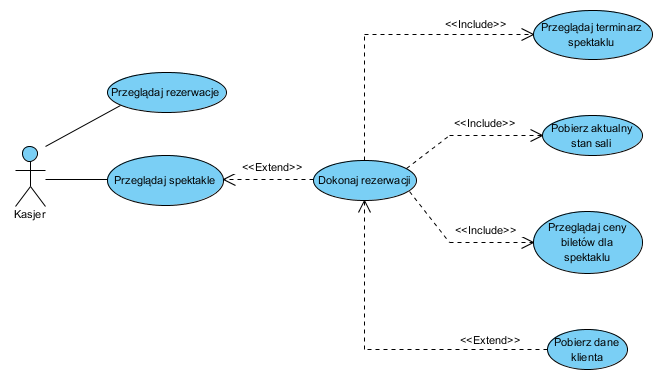
\includegraphics[width=0.75\textwidth]{images/diagram_pu.png}
	\caption{Diagram przypadków użycia}
	\label{fig:diagram_pu}
\end{figure}

W naszym systemie przewidziana została tylko jedna rola, jaką jest kasjer. Powinien on mieć możliwość przeglądania dokonanych rejestracji, a także wprowadzenia do systemu nowych. Przy opcji nowej rezerwacji, pracownik na podstawie informacji przekazanych przez klienta teatru, będzie miał możliwość wyboru sceny, terminu i wolnych miejsc na sali. Dokończenie procesu rezerwacji będzie wymagało wprowadzenia danych klienta. Jeżeli gość istnieje już w bazie danych, jego dane będzie można pobrać na podstawie adresu e-mail.

\section{Wymagania niefunkcjonalne}
Tworzona aplikacja ma być aplikacją webową. Umożliwi to użytkownikom dostęp do niej z niemal dowolnego urządzenia elektronicznego. Powinna być również responsywna, aby mimo różnych rozdzielczości ekranów zapewnić zadowalającą czytelność i funkcjonalność. Sam jej wygląd powinien być możliwie jak najprostszy, aby użytkownik nie czuł uczucia dyskomfortu podczas poruszania się po niej oraz by nie musiał poświęcić dużo czasu na nauczenie się jej obsługi.

\subsection{Wykorzystane technologie i narzędzia}
Dostęp  do  baz  danych  będzie  możliwy  za  pośrednictwem  odpowiednich  serwerów zarządzających bazami danych MySQL, a proces replikacji między nimi zostanie zrealizowany z wykorzystaniem programu MySQL Workbench. Ze stworzonego systemu baz danych będzie korzystać aplikacja webowa. Logika aplikacji została zaimplementowana przy użyciu języka Ruby wraz z biblioteką Sinatra. Natomiast warstwa prezentacji budowana była w HTML5, CSS3, Bootstrap, JavaScript i AngularJS. Do  specyfikacji  funkcji systemu wykorzystany zostanie język modelowania UML.

\subsection{Wymagania dotyczące rozmiaru bazy danych}
Baza danych stworzona zostanie do obsługi procesu rezerwacji biletów do teatru. Będzie to wymagało m.in. przechowywania danych o klientach, a także aktualnych rezerwacjach. Na stałe w bazie danych wprowadzone zostaną informacje o dostępnych salach. Informacje o aktualnie granych spektaklach, biletów na nie oraz terminarzu, nie będą wymagały dużej ilości miejsca. Najbardziej obciążone tabele bazy będą przechowywały dane klientów i rezerwacji. Zakładając, że w teatrze w danym okresie będzie granych kilka sztuk na różnych salach i w różnych terminach możemy spodziewać się, że dane o tym będą zapisane na co najmniej kilkaset rekordach. Jednakże informacje te będzie można usunąć po odbyciu się spektaklu, a więc baza danych nigdy nie powinna osiągnąć dużych rozmiarów.

\subsection{Wymagania dotyczące bezpieczeństwa systemu}
Najbardziej newralgiczne dane będą dotyczyły klientów teatru. W bazie będą przechowywane takie informacje jak numer telefonu, czy adres e-mail. Jednakże system został przeznaczony tylko dla pracowników teatru, a wcześniej wymienione dane nie są aż tak niebezpieczne by były dodatkowo szyfrowane. Dlatego przyjmujemy, że stworzony system nie wymaga dodatkowych zabezpieczeń. Za bezpieczeństwo wprowadzania danych odpowiadać będą zaimplementowane ograniczenia integralności bazy danych.

\section{Przyjęte założenia projektowe}
W projekcie będzie zrealizowany 3-warstwowy model komunikacji klient/serwer w postaci tzw. „cienkiego klienta” (Rys. \ref{fig:system-diagram}). Dostęp  do  aplikacji  realizującej  funkcje  biznesowe  będzie realizowany poprzez podanie adresu serwera WWW. W projekcie zostaną wykorzystywane niejednorodne, relacyjne bazy danych.  Dostęp  do  systemu baz  danych  zostanie zrealizowany  w  oparciu  o funkcje aplikacji. Komunikacja w systemie baz danych będzie przebiegała zgodnie z modelem master slave. Zapis będzie możliwy tylko na serwer z rolą mastera, natomiast odczyt będzie możliwy z wszystkich trzech serwerów bazodanowych. W celu zrównoważenia obciążenia wykorzystany zostanie Load Balancing.

\begin{figure}[!ht]
	\centering
	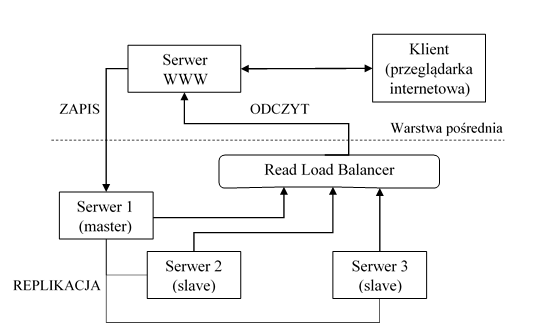
\includegraphics[width=0.7\textwidth]{images/struktura_systemu.png}
	\caption{Schemat systemu}
	\label{fig:system-diagram}
\end{figure}

\chapter{Projekt systemu}
W tym rozdziale przedstawiony został sposób w jaki zaprojektowana będzie aplikacja i jej baza danych.

\section{Projekt bazy danych}
Na etapie projektowania okazało się, że do właściwej pracy systemu będzie potrzebna baza danych składająca się z dziewięciu tabel.

\subsection{Model logiczny}
Model logiczny bazy danych został przedstawiony na rysunku \ref{fig:logical-data-model}.

\begin{figure}[!ht]
	\centering
	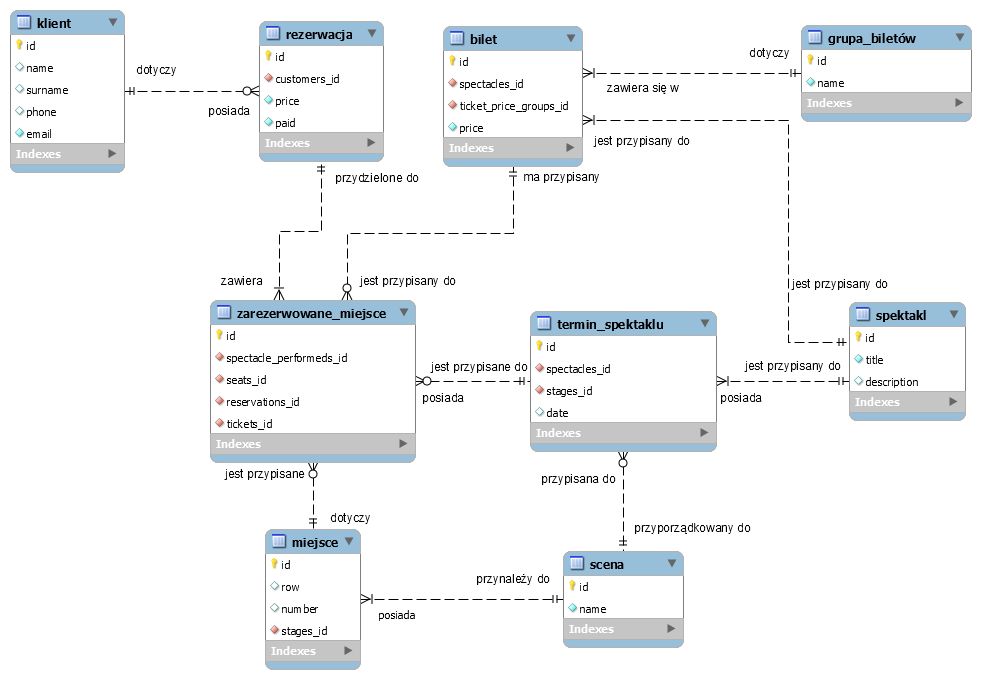
\includegraphics[width=\textwidth]{images/logiczny.png}
	\caption{Schemat logiczny bazy danych}
	\label{fig:logical-data-model}
\end{figure}

\subsection{Model fizyczny i ograniczenia integralności bazy danych}
Fizyczny model bazy danych (Rys. \ref{fig:physical-data-model}) został stworzony dla bazy MySQL. W modelu tym obok nazw kolumn w tabelach przedstawione zostały oczekiwane typy danych.

\begin{figure}[!ht]
	\centering
	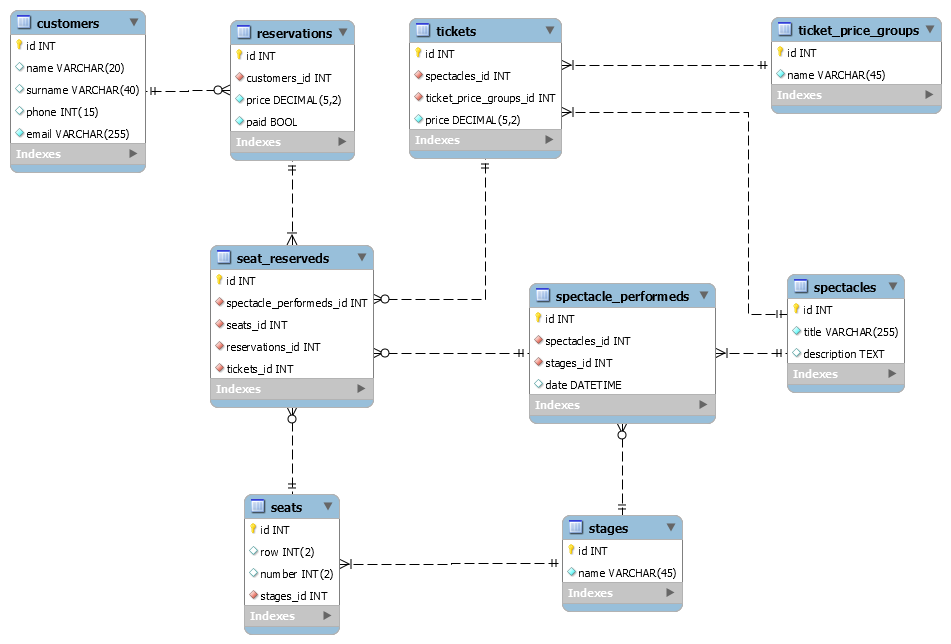
\includegraphics[width=\textwidth]{images/fizyczny.png}
	\caption{Schemat fizyczny bazy danych}
	\label{fig:physical-data-model}
\end{figure}

Dodatkowo na odpowiednie tabele nałożone zostały następujące ograniczenia integralności:
 
\begin{itemize}
	\item customers - na wszystkie kolumny not-null (NN), dodatkowo unique (U) na kolumnę email,
	\item reservations - na wszystkie kolumny NN,
	\item tickets - na wszystkie kolumny NN, dodatkowo U na parę kolumn spectacles\_id i ticket\_price\_groups\_id,
	\item ticket\_price\_groups - na wszystkie kolumny NN, na kolumnę name U,
	\item seat\_reserveds - na wszystkie kolumny NN, na parę spectacle\_performeds\_id i seats\_id U,
	\item spectacle\_performeds - na wszystkie kolumny NN, na parę stages\_id i date U,
	\item spectacles - na wszystkie kolumny NN,
	\item seats - na wszystkie kolumny NN, na grupę row, number i stages\_id U,
	\item stages - na wszystkie kolumny NN, na kolumnę name U.
	
\end{itemize}

\section{Projekt aplikacji użytkownika}
coś ???

\chapter{Implementacja systemu}
W tym rozdziale opisany został sposób w jaki stworzona została struktura bazy danych oraz jak wyglądała implementacja logiki biznesowej aplikacji.

\section{Realizacja bazy danych}
Baza danych została zaimplementowana w podejściu Database First. Została więc zaprojektowana, a następnie wdrożona za pomocą programu MySQL Workbench. Projektowanie odbywało się całkowicie w trybie graficznym. Następnie korzystając z narzędzi programu wygenerowany został skrypt sql tworzący bazę danych, który został wczytany do serwerów typu slave.

\section{Realizacja mechanizmu replikacji}
Replikacja baz danych została przeprowadzona z wykorzystaniem programu MySQL Workbench. Przed przystąpieniem do jakich kolwiek czynności należy upewnić czy wszystkie bazy posiadają dokładnie taką samą strukturę. W naszym systemie struktura została zaprojektowana, a następnie wprowadzona na serwerze typu master. Po sprawdzeniu poprawności jej działania, korzystając z wcześniej wymienionego programu, struktura bazy została wyeksportowana w postaci skryptu sql. Następnie skrypt ten został wczytany na serwery typu slave. Opcja eksportu i importu bazy danych znajduje się w lewym menu programu w grupie "Management" (Rys. \ref{fig:wb-management}).

\begin{figure}[!ht]
	\centering
	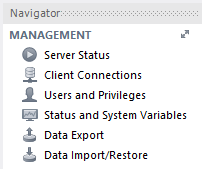
\includegraphics[width=0.3\textwidth]{images/wb_management.png}
	\caption{Grupa opcji Management programu MySQL Workbench}
	\label{fig:wb-management}
\end{figure}

Następnie dla celów replikacji w bazie danych typu master stworzony został użytkownik replication\_user o uprawnieniach przedstawionych na rysunku \ref{fig:wb-users-privileges}.

\begin{figure}[!ht]
	\centering
	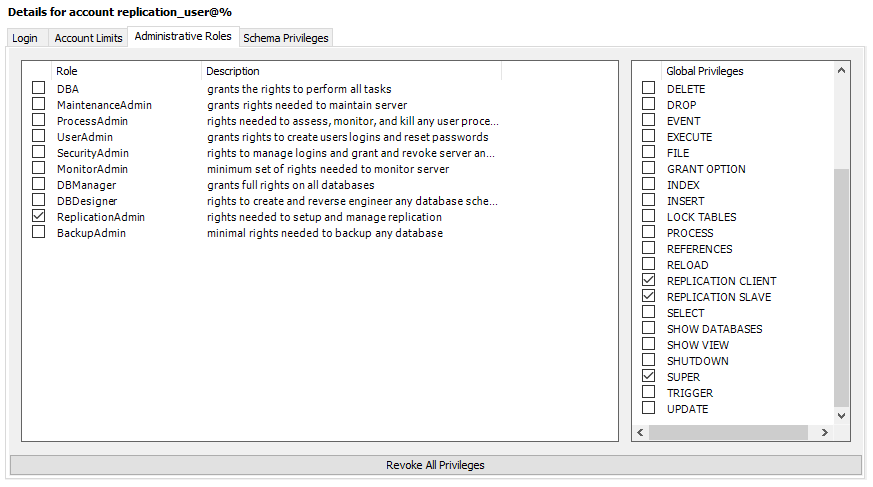
\includegraphics[width=0.9\textwidth]{images/wb_users_privileges.png}
	\caption{Uprawnienia użytkownika replication\_user}
	\label{fig:wb-users-privileges}
\end{figure}

Następnie wybierając opcję "Options File" (Rys. \ref{fig:wb-instance}) przechodzi się do ustawień serwera bazy danych. Na serwerze mastera należało aktywować i ustawić następujące opcje:

\begin{itemize}
	\item server\_id na 1,
	\item binlog-do-db na nazwę bazy danych theatre,
	\item log-bin na mysql55-bin.
\end{itemize}

Pierwsza opcja dotyczy nadania serwerowi numeru id, dzięki czemu możliwa będzie komunikacja z innymi serwerami. W drugiej określa się bazę danych jaka będzie podlegać replikacji. W ostatniej ustawia się nazwę dla pliku w którym będą przechowywane logi z działania serwera.

\begin{figure}[!ht]
	\centering
	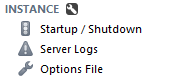
\includegraphics[width=0.3\textwidth]{images/wb_instance.png}
	\caption{Grupa opcji Instance programu MySQL Workbench}
	\label{fig:wb-instance}
\end{figure}

Po zatwierdzeniu wprowadzonych danych warto zrestartować serwer, a następnie zweryfikować status mastera za pomocą odpowiedniej komendy, przedstawionej wraz z wynikiem na rysunku \ref{fig:wb-master-status}.

\begin{figure}[!ht]
	\centering
	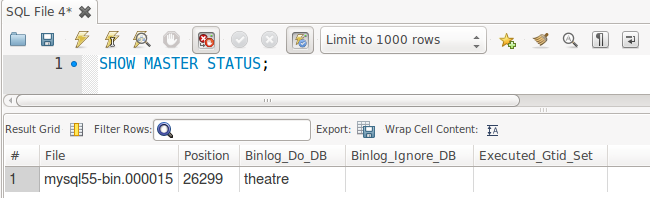
\includegraphics[width=0.8\textwidth]{images/wb_master_status.png}
	\caption{Wyświetlenie statusu serwera typu master}
	\label{fig:wb-master-status}
\end{figure}

Następnie należy wykonać konfigurację serwerów typu slave. Ponownie wybieramy opcję "Options File" (Rys. \ref{fig:wb-instance}), gdzie należy ustawić następujące opcje:

\begin{itemize}
	\item server\_id na liczbę większą od 1,
	\item replicate-do-db na nazwę bazy danych theatre.
\end{itemize}

Tak jak przy masterze ustawiane jest id oraz opcja replicate-do-db wskazująca bazę jaka ma być replikowana. Po zatwierdzeniu wprowadzonych danych należy zrestartować serwer. Serwer typu slave nie jest jeszcze poprawnie ustawiony, należy wykonać jeszcze kilka komend, które wraz z wynikiem przedstawione zostały na rysunku \ref{fig:wb-slave-status-cmd}.

\begin{figure}[!ht]
	\centering
	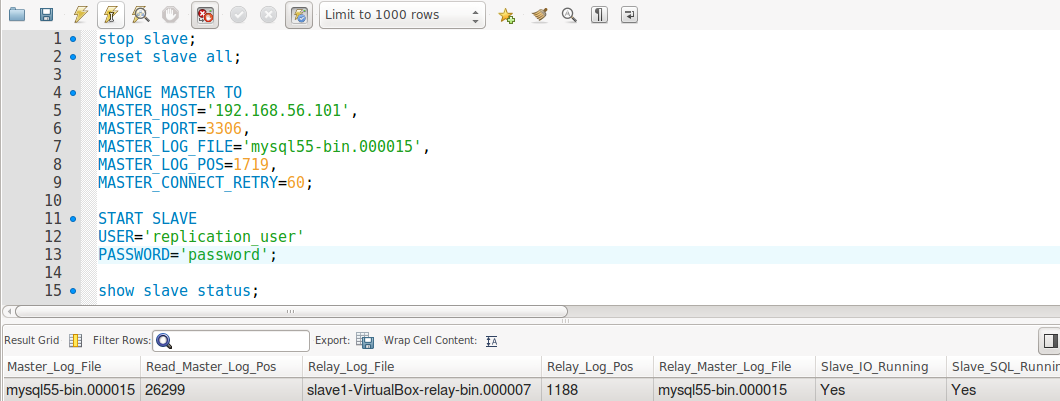
\includegraphics[width=\textwidth]{images/wb_slave_status_cmd.png}
	\caption{Ustawienie oraz sprawdzenie statusu serwera typu slave}
	\label{fig:wb-slave-status-cmd}
\end{figure}

Na początku wykonywane są komendy odpowiedzialne za ewentualne zatrzymanie działania slave'a i zresetowanie wszelkich ustawionych na nim opcji. W następnej komendzie opcja MASTER\_LOG\_FILE i MASTER\_LOG\_POS to nazwa pliku i pozycja jaką można odczytać po wyświetleniu statusu mastera (Rys. \ref{fig:wb-master-status}). Dalej serwer jest uruchamiany z wykorzystaniem użytkownika replication\_user. Na samym końcu umieszczona została komenda wyświetlająca aktualny status serwera typu slave. O prawidłowości wykonanej replikacji świadczą kolumny Slave\_IO\_Running i Slave\_SQL\_Running, które powinny być ustawione na wartość YES.

\section{Realizacja elementów aplikacji}

\subsection{Realizacja części klienckiej}
Część kliencka została zrealizowana jako aplikacja webowa z wykorzystaniem przede wszystkim frameworków AngularJS i Bootstrap. Pierwszy z nich odpowiedzialny był za połączenie z serwerem, przygotowywanie danych do wyświetlenia, operacji na nich, a także walidacji. Drugi został wykorzystany w celu lepszej organizacji treści na stronie i do utrzymania responsywności strony.

Przy wejściu do aplikacji pokazuje się strona startowa (Rys. \ref{fig:main-page}). Z niej użytkownik systemu może przejść do panelu rezerwacji, wciskając widoczny przycisk. Po wykonaniu tej czynności wyświetla się strona z listą spektakli (Rys. \ref{fig:spectacles}). Po wyborze jednego z nich przechodzi się do następnego widoku (Rys. \ref{fig:stages}). 

W tym momencie pracownik ma możliwość zarezerwowania biletów dla klienta. Na początku powinien wybrać scenę i datę kiedy ma odbyć się spektakl. Po wykonaniu tego na stronie pojawi się model przedstawiający rozłożenie miejsc na sali. Siedzeniom przypisane zostały odpowiednie numery i różne kolory. Kolorem zielonym oznaczone zostały dostępne miejsca. Kolorem siwym wyróżniono miejsca już przez kogoś zarezerwowane. Natomiast kolorem czerwonym oznaczane są miejsca wybrane dla aktualnie obsługiwanego klienta. Poniżej sceny widoczna jest sekcja "Wybrane miejsca", gdzie ponownie wypisane zostały wybrane miejsca, ale dodatkowo do każdego z nich należy przypisać bilet. W prezentowanym przypadku mamy doczynienie z biletem normalnym i ulgowym. Jednakże nazwy i oczywiście ceny dla biletów można definiować własne. Po wyborze biletów należy już tylko uzupełnić dane o kliencie. Wszystkie te dane są odpowiednio walidowane, a w przypadku niepoprawnie wprowadzonych danych, użytkownikowi wyświetlany jest krótki komunikat tuż przy błędnym polu. Jeżeli klient dokonywał wcześniej jakieś inne rezerwacje, jego dane powinny znajdować się w systemie. W celu ich pobrania, pod polem "Email" umieszczony został link, który pobiera informację o kliencie na podstawie wprowadzonego adresu e-mail. Po uzupełnieniu wszystkich wymaganych informacji należy kliknąć przycisk "Zarezerwuj". Po krótkiej chwili pod formularzem powinien pojawić się komunikat czy rezerwacja się powiodła. 

Ostatni widok jaki został zaimplementowany to widok z listą aktualnie dokonanych rezerwacji (Rys. \ref{fig:reservations}). W lewej kolumnie znajduje się wspomniana lista, a w prawej szczegóły o wybranej rezerwacji.


\begin{figure}[!ht]
	\centering
	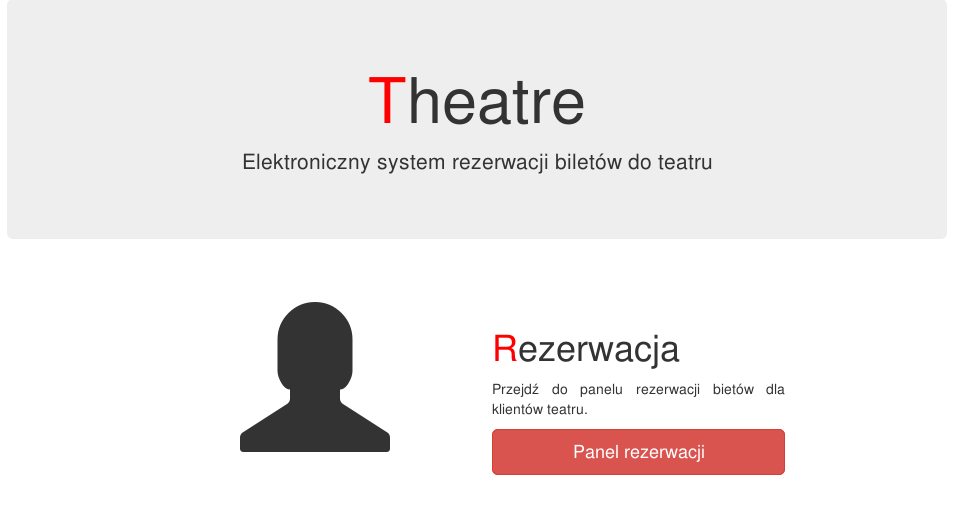
\includegraphics[width=\textwidth]{images/main_page.png}
	\caption{Strona główna aplikacji}
	\label{fig:main-page}
\end{figure}

\begin{figure}[!ht]
	\centering
	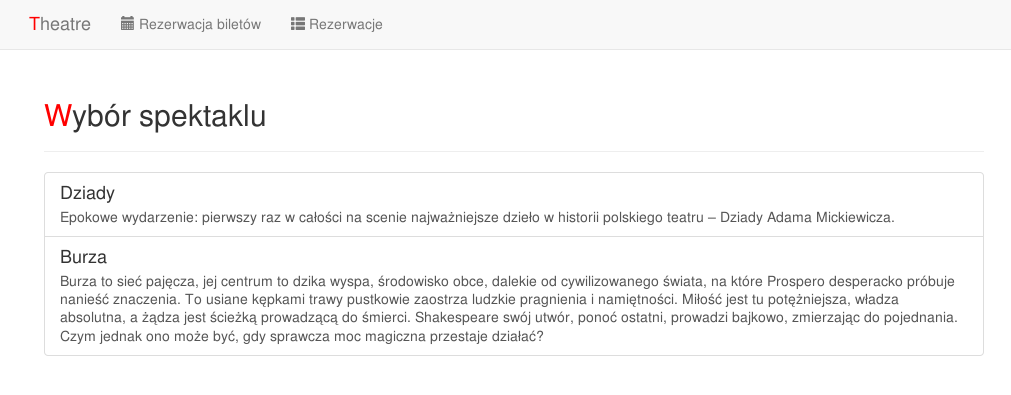
\includegraphics[width=\textwidth]{images/spectacles.png}
	\caption{Widok z listą spektakli}
	\label{fig:spectacles}
\end{figure}

\begin{figure}[!ht]
	\centering
	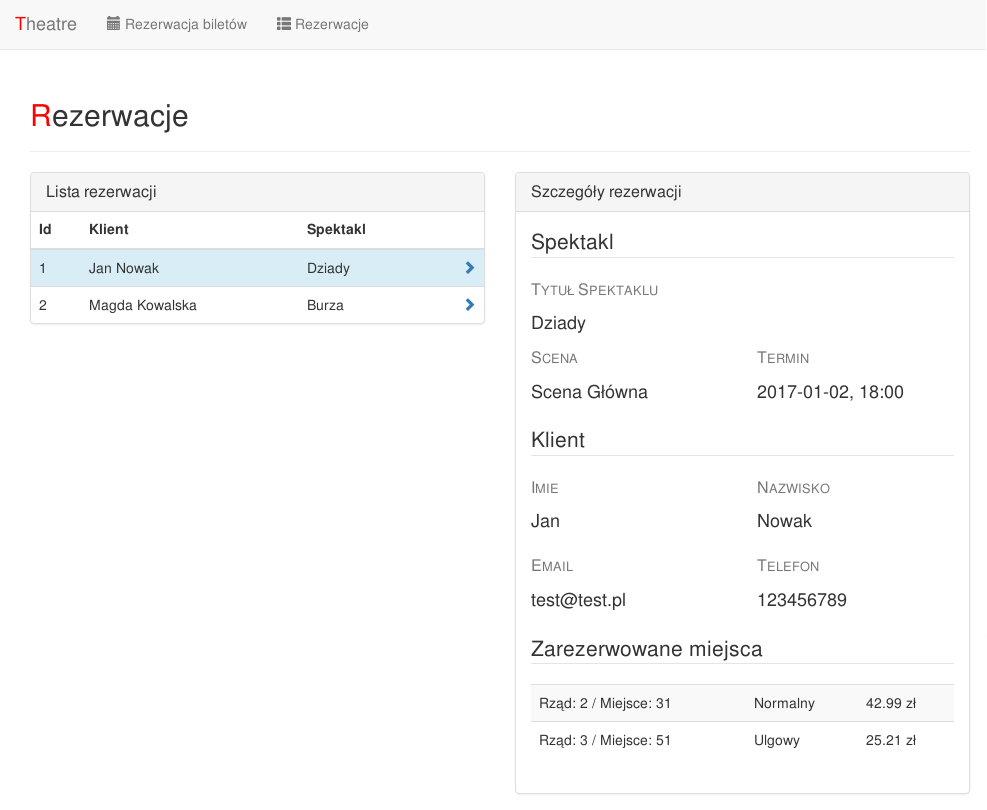
\includegraphics[width=\textwidth]{images/reservations.png}
	\caption{Widok z listą dokonanych rezerwacji}
	\label{fig:reservations}
\end{figure}

\begin{figure}[!ht]
	\centering
	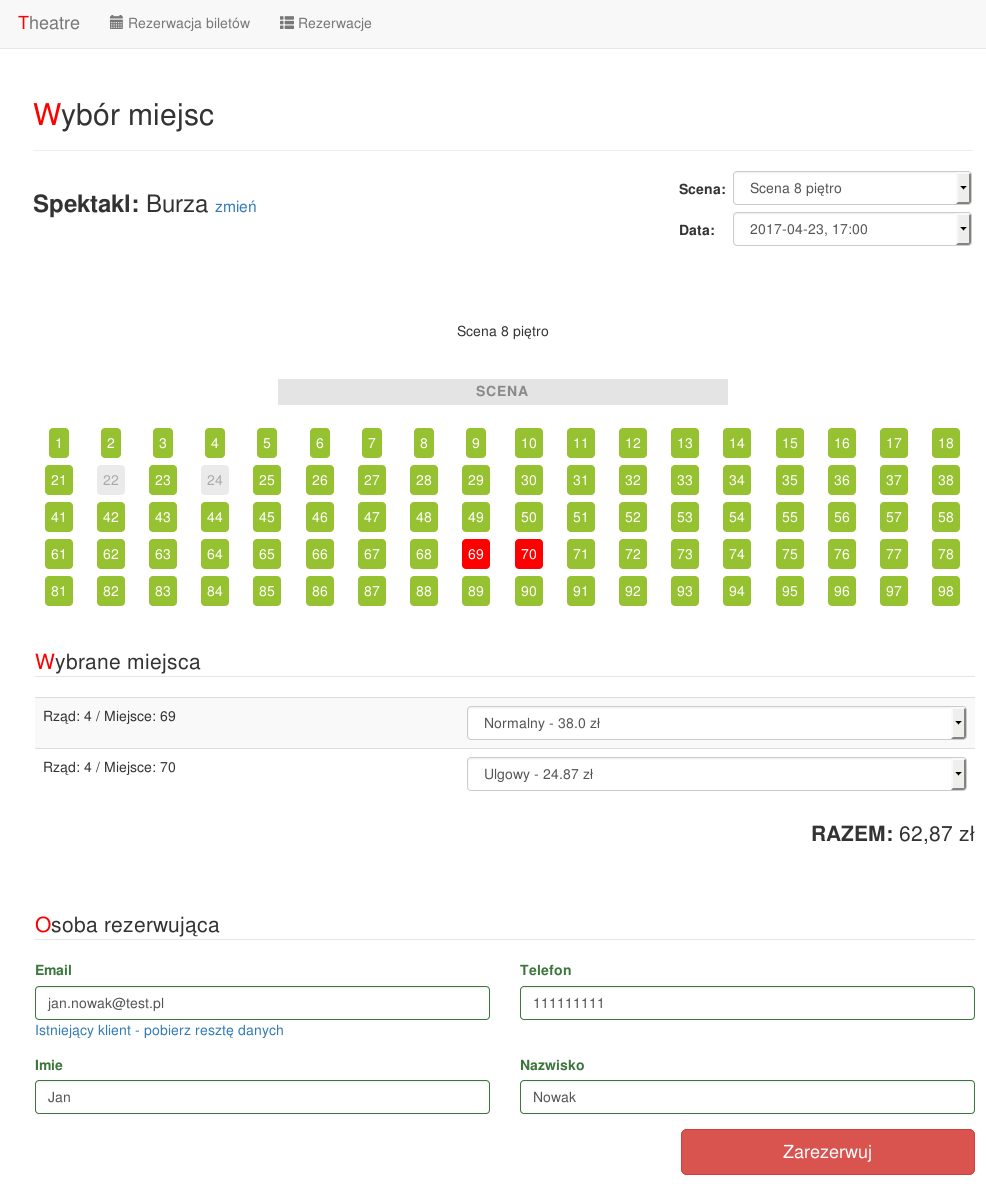
\includegraphics[width=\textwidth]{images/stages.png}
	\caption{Widok przedstawiający przykładową rezerwację}
	\label{fig:stages}
\end{figure}

\chapter{Testowanie systemu}
Testowanie zastało opisane w dwóch podrozdziałach dotyczących odpowiednio testowania działania systemu i testowania mechanizmów bezpieczeństwa bazy danych.

\section{Testowanie poprawności działania systemu}
W celu sprawdzenia poprawności działania systemu przeprowadzono proces rezerwacji biletów dla fikcyjnego klienta teatru. Proces ten zakończył się prawidło. Oznacza to, żę widoczne na rysunku \ref{fig:app-reservation-success} dane klienta powinny zostać zapisane zarówno w bazie trzymanej na serwerze typu master, jak i w bazach dwóch pozostałych serwerów typu slave. W celu sprawdzenia tego wykonano odpowiednią komendę na wszystkich serwerach i na wszystkich otrzymano taki sam wynik zaprezentowany na rysunku \ref{fig:app-db-show-clients}.

\begin{figure}[!ht]
	\centering
	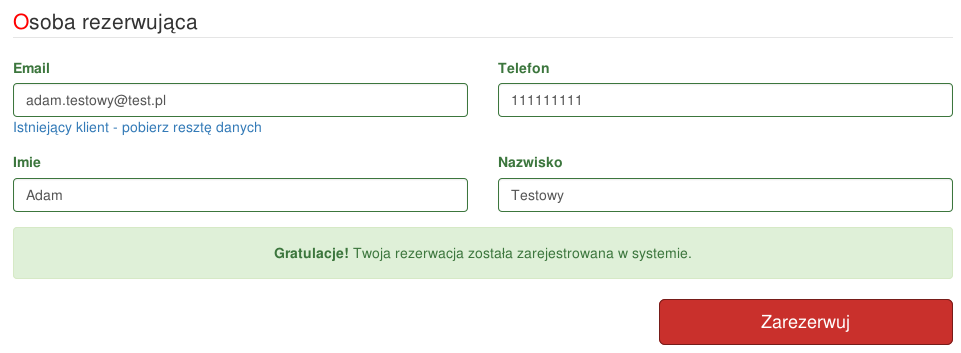
\includegraphics[width=0.8\textwidth]{images/app_reservation_success.png}
	\caption{Potwierdzenie wykonania rezerwacji}
	\label{fig:app-reservation-success}
\end{figure}

\begin{figure}[!ht]
	\centering
	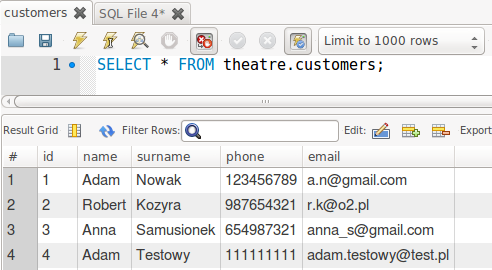
\includegraphics[width=0.5\textwidth]{images/app_db_show_clients.png}
	\caption{Potwierdzenie wykonania rezerwacji}
	\label{fig:app-db-show-clients}
\end{figure}


\section{Testowanie mechanizmów bezpieczeństwa bazy danych}
Bezpieczeństwo bazy danych może zostać pokazane na podstawie tabeli seats\_reserved, która odpowiada za przechowywanie informacji o zarejestrowanych miejscach. W tej tabeli zostało ustawione ograniczenie niepozwalające wprowadzić rezerwację na już zajęte miejsce dla danego wystawienia spektaklu. Aktualne wypełnienie bazy danych został przedstawione na rysunku \ref{fig:app_db_seats_reserved}. Dla sprawdzenia omówionych mechanizmów bezpieczeństwa została wykonana odpowiednia komenda. Jej treść oraz zwrócony wynik zostały zawarte na rysunku \ref{fig:app_db_insert_fail}. Jak widać ograniczenie ui\_seat\_spectacle\_performed zwraca błąd nie pozwalając na dodanie niepoprawnych danych do bazy.

\begin{figure}[!ht]
	\centering
	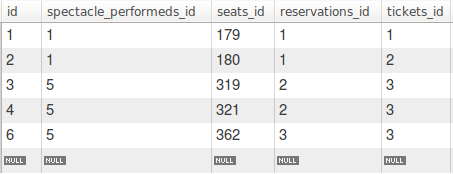
\includegraphics[width=0.6\textwidth]{images/app_db_seats_reserved.png}
	\caption{Zawartość tabeli seats\_reserved}
	\label{fig:app_db_seats_reserved}
\end{figure}

\begin{figure}[!ht]
	\centering
	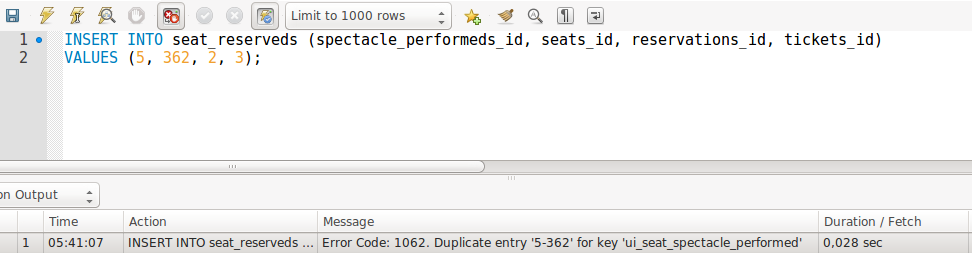
\includegraphics[width=\textwidth]{images/app_db_insert_fail.png}
	\caption{Próba zapisania dwóch osób na jedno miejsce zakończona niepowodzeniem}
	\label{fig:app_db_insert_fail}
\end{figure}

\section{Wnioski z testów}
coś

\chapter{Podsumowanie pracy}
voluptas sit, aspernatur aut odit aut fugit, sed quia consequuntur magni dolores eos, qui ratione voluptatem sequi nesciunt, neque porro quisquam est, qui dolorem ipsum, quia dolor sit, amet, consectetur, adipisci velit, sed quia non numquam eius modi tempora incidunt, ut labore et dolore magnam aliquam quaerat voluptatem. Ut enim ad minima veniam, quis nostrum exercitationem ullam corporis suscipit laboriosam, nisi ut aliquid ex ea commodi consequatur? Quis autem vel eum iure reprehenderit, qui in ea voluptate velit esse, quam nihil molestiae consequatur, vel illum, qui dolorem eum fugiat, quo voluptas nulla pariatur?

Sed ut perspiciatis, unde omnis iste natus error sit voluptatem accusantium doloremque laudantium, totam rem aperiam eaque ipsa, quae ab illo inventore veritatis et quasi architecto beatae vitae dicta sunt, explicabo. Nemo enim ipsam voluptatem, quia voluptas sit, aspernatur aut odit aut fugit, sed quia consequuntur magni dolores eos, qui ratione voluptatem sequi nesciunt, neque porro quisquam est, qui dolorem ipsum, quia dolor sit, amet, consectetur, adipisci velit, sed quia non numquam eius modi tempora incidunt, ut labore et dolore magnam aliquam quaerat voluptatem. Ut enim ad minima veniam, quis nostrum exercitationem ullam corporis suscipit laboriosam, nisi ut aliquid ex ea commodi consequatur? Quis autem vel eum iure reprehenderit, qui in ea voluptate velit esse, quam nihil molestiae consequatur, vel illum, qui dolorem evoluptas sit, aspernatur aut odit aut fugit, sed quia consequuntur magni dolores eos, qui ratione voluptatem sequi nesciunt, neque porro quisquam est, qui dolorem ipsum, quia dolor sit, amet, consectetur, adipisci velit, sed quia non numquam eius modi tempora incidunt, ut labore et dolore magnam aliquam quaerat voluptatem. Ut enim ad minima veniam, quis nostrum exercitationem ullam corporis suscipit laboriosam, nisi ut aliquid ex ea commodi consequatur? Quis autem vel eum iure reprehenderit, qui in ea voluptate velit esse, quam nihil molestiae consequatur, vel illum, qui dolorem eum fugiat, quo voluptas nulla pariatur?

Sed ut perspiciatis, unde omnis iste natus error sit voluptatem accusantium doloremque laudantium, totam rem aperiam eaque ipsa, quae ab illo inventore veritatis et quasi architecto beatae vitae dicta sunt, explicabo. Nemo enim ipsam voluptatem, quia voluptas sit, aspernatur aut odit aut fugit, sed quia consequuntur magni dolores eos, qui ratione voluptatem sequi nesciunt, neque porro quisquam est, qui dolorem ipsum, quia dolor sit, amet, consectetur, adipisci velit, sed quia non numquam eius modi tempora incidunt, ut labore et dolore magnam aliquam quaerat voluptatem. Ut enim ad minima veniam, quis nostrum exercitationem ullam corporis suscipit laboriosam, nisi ut aliquid ex ea commodi consequatur? Quis autem vel eum iure reprehenderit, qui in ea voluptate velit esse, quam nihil molestiae consequatur, vel illum, qui dolorem evoluptas sit, aspernatur aut odit aut fugit, sed quia consequuntur magni dolores eos, qui ratione voluptatem sequi nesciunt, neque porro quisquam est, qui dolorem ipsum, quia dolor sit, amet, consectetur, adipisci velit, sed quia non numquam eius modi tempora incidunt, ut labore et dolore magnam aliquam quaerat voluptatem. Ut enim ad minima veniam, quis nostrum exercitationem ullam corporis suscipit laboriosam, nisi ut aliquid ex ea commodi consequatur? Quis autem vel eum iure reprehenderit, qui in ea voluptate velit esse, quam nihil molestiae consequatur, vel illum, qui dolorem eum fugiat, quo voluptas nulla pariatur?

Sed ut perspiciatis, unde omnis iste natus error sit voluptatem accusantium doloremque laudantium, totam rem aperiam eaque ipsa, quae ab illo inventore veritatis et quasi architecto beatae vitae dicta sunt, explicabo. Nemo enim ipsam voluptatem, quia voluptas sit, aspernatur aut odit aut fugit, sed quia consequuntur magni dolores eos, qui ratione voluptatem sequi nesciunt, neque porro quisquam est, qui dolorem ipsum, quia dolor sit, amet, consectetur, adipisci velit, sed quia non numquam eius modi tempora incidunt, ut labore et dolore magnam aliquam quaerat voluptatem. Ut enim ad minima veniam, quis nostrum exercitationem ullam corporis suscipit laboriosam, nisi ut aliquid ex ea commodi consequatur? Quis autem vel eum iure reprehenderit, qui in ea voluptate velit esse, quam nihil molestiae consequatur, vel illum, qui dolorem eję danych na stronie
internetowej, co zwiększa liczbę zastosowań systemu.
 
Dalszy rozwój projektu może zakładać:
\begin{itemize}
\item projekt obwodfgsgfsgudowy ursządzenigsdo-nadawczego,
\item optymalizagfdsgsgsfgso mają być
wyświetlane pomiary,
\item możliwsgfsdgfsów do pliku.
\item powiadamianie usgdfgsdfgczeniu mierzonej wielkości
fizycznej,
\item sterowaniesdgsdfgscję internetową.
\end{itemize}
 %utworzenie w
                                             %spisietresci pozycji
                                             %Bibliografia
  \begin{thebibliography}{9}
\addcontentsline{toc}{chapter}{Bibliografia}

  \bibitem{rfc2616} {\em Hypertext Transfer Protocol -- HTTP/1.1} 1999: 
  https://tools.ietf.org/html/rfc2616 (dostęp 09.12.2015 r.)

  \bibitem{ajax} {\em XMLHttpRequest Living Standard} 25.11.2015 r.: 
  https://xhr.spec.whatwg.org/ (dostęp 11.12.2015 r.)

  \end{thebibliography}
%\bibliography{bibliografia} % wstawia bibliografię korzystając z pliku
                            % bibliografia.bib - dotyczy BibTeXa,
                            % jeżeli nie korzystamy z BibTeXa należy
                            % użyć otoczenia thebibliography

%opcjonalnie może się tu pojawić spis rysunków i tabel
\listoffigures
\addcontentsline{toc}{chapter}{Spis rysunków}
 \listoftables
\addcontentsline{toc}{chapter}{Spis tabel}
% \listoflistings
 \lstlistoflistings
 \addcontentsline{toc}{chapter}{Spis listingów}

\end{document}
